\chapter{Introduction}

%This chapter must contain presentation of 

%\begin{itemize}
%	\item context
%	\item problematic
%	\item company  activities
%	\item internship context 
%\end{itemize}

%The following organization can be used.



\section{Context}
%Noise pollution is the disturb or loud noise may effected the activity or health of peole or
%animal in life. Most of outdoor noise is mainly caused by machines and transportation
%systems, motorbike engines, airplanes, and trains. Outdoor noise meaning is the
%environmental noise: Urban planning or industrial areas are representation examples
%Nowdays, noise levels can be main cause by cardiovascular illness or coronary artery in
%human. For animals, noise can increase the count of death ,bad effected to reproduction
%and hearing loss



Moreover, noise also appears in the images. Image noise is created by the sensor and
circuitry from scanner or digital camera. Film grain and noise of an ideal photon detector
are one of cause. So brightness or color information in images will be changed. Image noise is not same as normal image that have many different information.

\

Although camera technology is very improve over the past
decade, it still has not totally remove noise for images. So now, researchers still find to
way which improve about camera to have better images is better. Noise can appear in our
photo for different reasons. Noise signal with the light signal increase when high ISO is used.  Camera need lighter to creat good image, but noise also more appear. When the image sensor is hot, photons evacuate from the images and damage other images. Long exposures is one of cause to appear noise in image becaue the sensor open to have more image information and electrical noise will appear.

\

Denoise is a process of remove noise to images. There are ways to noise removal in image, data. With image denoise model is completely remove noise and protect edges. Basically, there are two types of models : linear and non-liner. Linear models is removing models is the speed also as limitations of itself. It’s not able to protect edges which are recognized as discontinuities in the image. It's not able to protect edges which are recognized as discontinuities in the image. So, blur edges could appear in images.

\

On the other hand, non-linear models can solve edges problem much better than linear models. We suppose non-linear image denoising model use the Total Variation (TV)- filter. Denoise a degraded image X by X = S + N, meaning sum of S (original image) and N (Gaussian noise) with unknown value. We call unknown value is ($\sigma$) which is the standard deviation of the distribution.





\vspace*{1cm}

%\subsection{Company activities}


%\vspace*{1cm}

\subsection{Internship context}
One of the major problems in document digitalization is noise. Image noise is random (not present in the object imaged) when it change brightness level or color in images. It can be generated in many scanning steps, such as grayscaling or thresholding. It can also be caused by image lossy compression algorithms, such as JPEG’s discrete cosine transformation and thresholding. Noise is one of the main factors contributing to degratation of accuracy in optical character recognition of the scanned documents, a process aiming at providing a high semantic description of the content of the document. At ICTLab, we have been dealing with scanned document in the context of project ARCHIVES. A good noise evaluation and reduction algorithm will improve our document analysis (including optical character recognition) results. We are going to survey different denoising methods. From this, we will compare result of methods as : Median filter, Average filter, Gaussian filter, Wiener filter by we are using PSNR and MSE. Based on the quality characteristics of two methods MSE \& PSNR to compare. Created comparison table and showed image result, finally we will know method is the best. Although, images processing has many method to remove noise but due to limited time, many other methods can not be explored and the results are only relative.


\vspace*{1cm}



\section{Problematic}
We have two problems in this topic:





\subsection*{Noise}
\begin{itemize}
\item Noise is the cause of errors from image when in pixel values
that do not reflect the true intensities of the real scene.

\item ISO values: a standard of absolute sensitivity to light.
\end{itemize}
\vspace{0.3cm}

\textbf{There are 3 type of noise:}
\vspace{0.3cm}

Fixed pattern noise appears during long exposures. When the camera is working for long periods of time and it heats up, the sensor starts to produce these strange dots of color in our image. Our camera is hotter, more fixed pattern noise will appear. Fixed pattern noise usually easier to remove since it is repeatable. A camera just has to know the pattern and it can remove fixed pattern.
\vspace{0.5cm}

\begin{center}
	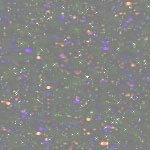
\includegraphics{fix.png}

Long Exposure

Low ISO Speed
\end{center}
\vspace{0.5cm}

%\newpage
%\item Random Noise

Random noise may be the most common image noise. Random noise appears whenever we are using high ISO
values. ISO has mean is a standard which describes its absolute sensitivity to light. 
Quality of camera is good when it remove random noise through software. Example: Neat Image and Noise Ninja programs, they can be removing noise and protect image information. When technology continues to
improve, we can shoot in low light situation.

\begin{center}
	
\includegraphics{random.png}

Short Exposure

High ISO Speed
\end{center}



%\item Banding Noise

Banding noise is dependent on what type of camera we are using. With high end cameras, we have never seen banding noise. Banding noise will appear when lower quality photograph are shot with higher
ISO value.
There are causes help banding noise appear: in the dark of photos or increase exposure too much and
digitally make a photograph too bright. We may also see more banding noise in certain white balances which is the process of removing unreal color.
\vspace{0.5cm}

\begin{center}
	
\includegraphics{banding.png}

Susceptible Camera

Brightened Shadows
\end{center}

%\end{itemize}

\subsection*{Denoise}

Noise removal is very important task in image processing. It will help to remove the noise from the image and rebuild to original image is the best quality. In modern digital image processing, data denoising is a hard problem and it used to application areas. Noise removal is popular solution for photography or improve the image was degraded.

\

Filtering is technique which can be decreasing or increasing an image.It's processed value for current pixel will depends itself and surrounding pixels . The value of any pixel in the output image is used by applying  algorithms to the values of the pixels in the place which corresponding input pixel.

\

Follow Image Processing, there are 4 types of filtering :

\begin{itemize}
\item Median Filter.

The median filter method is very popular in image processing and it protects edges while removing noise in certain environment
\item Average Filter.

Average filtering is simply to replace each pixel value in an image with the average value of its area, including itself. Its meaning is remove pixel values which aren't types of their environment.

\item Gaussian Filter.

Gaussian filters never go through to function input while minimizing the time.

 
\item Wiener Filter

The Wiener filter decreases the mean square error between the random process and the desired process.


\end{itemize} 
%\end{itemize}

%\vspace*{1cm}











\section{Report organization}
In this report, we have 5 chapters as below :
\begin{itemize}
\item Chapter 1 : Introduction

This chapter included presentation of: Context and Problematic. Context is the part that describe about problems and solutions through this report. Problematic is determination and analysis to problem in this topic. 
\item  Chapter 2 : State Of The Art

Collected different papers addressing the same topics of internship. Next to explain the work published, by giving the context of the work, the main idea, the main results. From this, we can learn more about how to present and solve problems of the authors. 

\item  Chapter 3 : Contribution

In this part, proposed method to solve the problem in the introduction chapter. Beside this, explain method/algorithm/system in proposition.

\item  Chapter 4 \& 5 : Result \& Conclusion

This part include the result of the method/algoritm/system developed. Moreover, it contain comparisons table,  figures, graphics and comment. Recall the problematic, methods used,  contribution, results obtained and future developed.

\end{itemize}
